\documentclass[preview]{standalone}

\usepackage{amsmath}
\usepackage{amssymb}
\usepackage{stellar}
\usepackage{wrapfig}
\usepackage{bettelini}

\hypersetup{
    colorlinks=true,
    linkcolor=black,
    urlcolor=blue,
    pdftitle={Stellar},
    pdfpagemode=FullScreen,
}

\begin{document}

\title{Geografia economica}
\id{geoeconomica-transizione-demografica}
\genpage

\section{La transizione demografica}

\begin{snippet}{56415993-9963-4be7-8c4f-48791fa9f8d4}
    Da analisi dei dati della popolazione dei paesi industrializzati,
    emerge un modello di crescita comune:
    il modello della \textbf{transizione demografica}.
    
    La transizione consiste in un calo, temporaneamente sfasato,
    dei tassi di mortalità e natalità.
\end{snippet}

\includesnpt[width=80\%|src=/snippet/static/fasi-demografia.png]{centered-img}

\section{Piramidi della popolazione}

\begin{snippet}{piramidi-demografiche-tipi}
    %=== PIRAMIDE A BASE ALLARGATA ===
    \setlength{\intextsep}{0pt}%
    \begin{wrapfigure}{r}{.35\textwidth}
        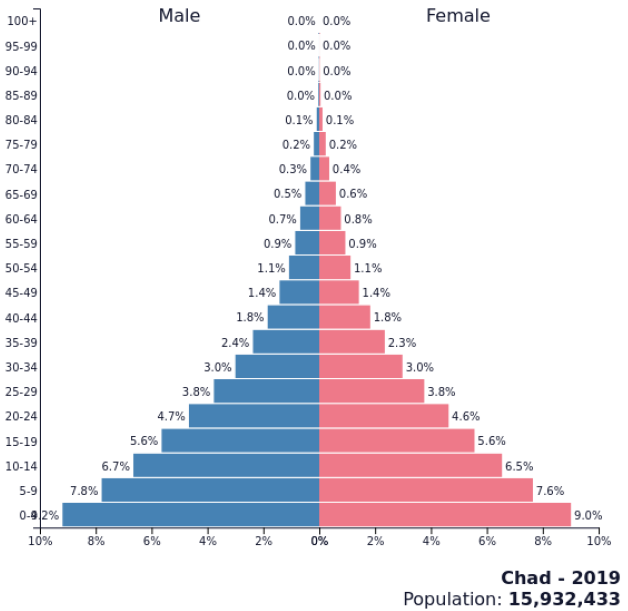
\includegraphics[width=.35\textwidth]{resources/piramide-demografica-base-allargata.png}
        \vspace{-0.5cm}
    \end{wrapfigure}
    \textbf{Piramide a base allargata}

    \begin{itemize}
        \item Tasso di natalità alto (ev. in aumento);
        \item Tasso di mortalità omogeneo già dalle fasce più giovani;
        \item Popolazione in (leggera) crescita, alta percentuale giovani.
    \end{itemize}
    \wrapfill

    %=== PIRAMIDE ===
    \setlength{\intextsep}{0pt}%
    \begin{wrapfigure}{l}{.35\textwidth}
        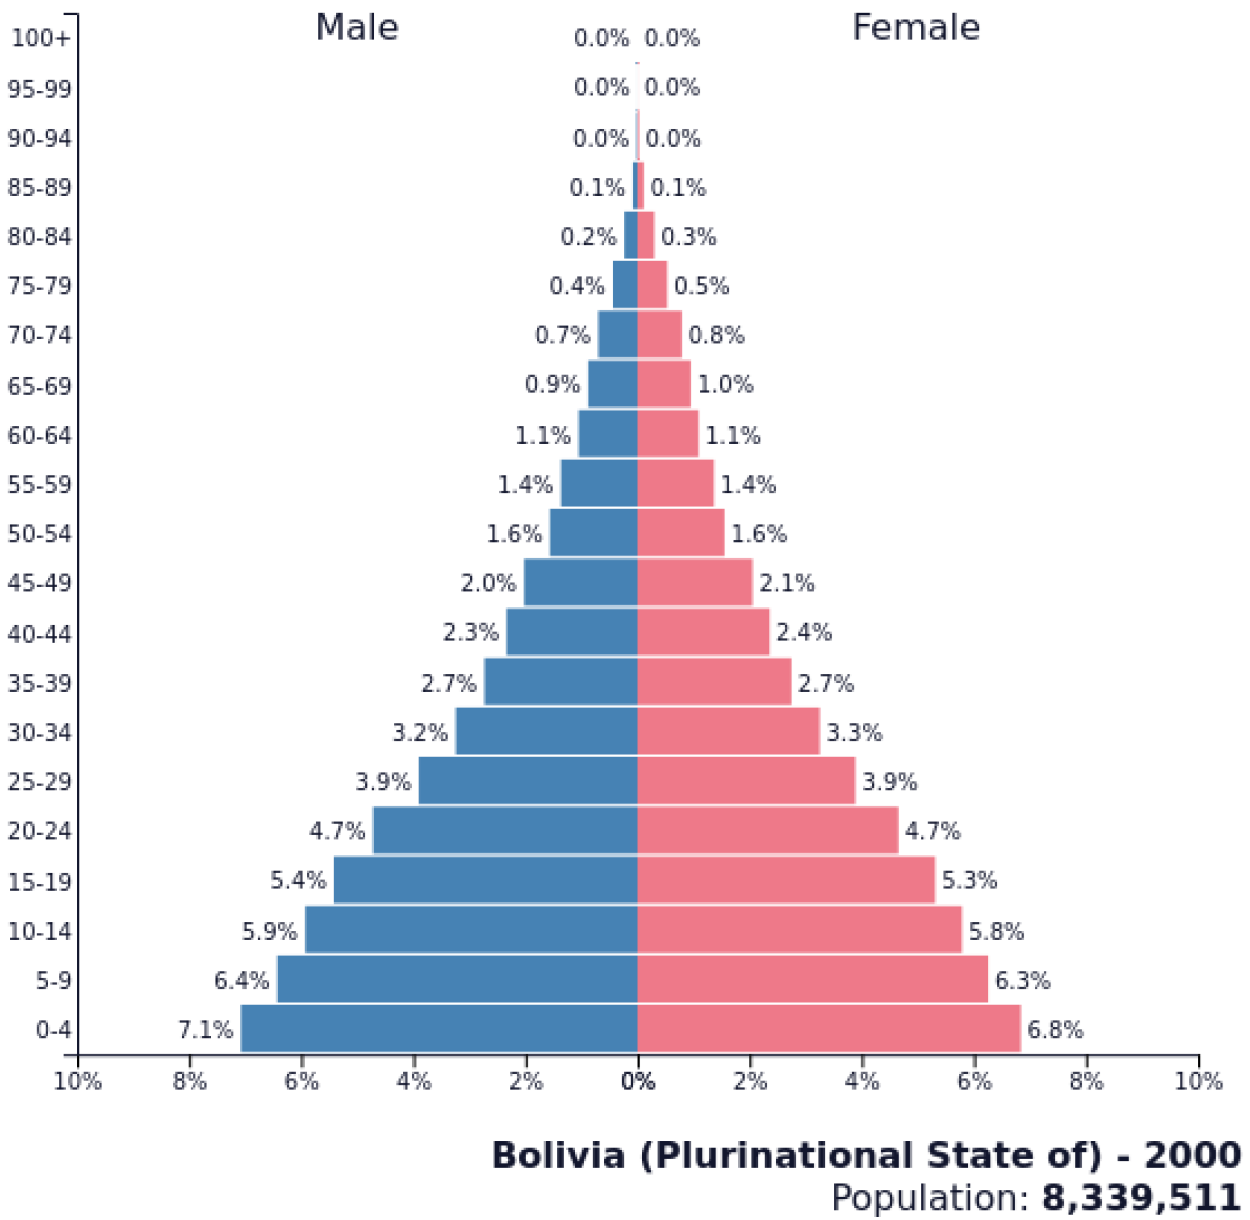
\includegraphics[width=.35\textwidth]{resources/piramide-demografica.png}
        \vspace{-0.5cm}
    \end{wrapfigure}
    \textbf{Piramide}

    \begin{itemize}
        \item Tasso di natalità alto;
        \item Tasso di mortalità in diminuzione, distribuito omogeneamente su tutte le fasce;
        \item Popolazione in (forte) aumento.
    \end{itemize}
    \wrapfill

    %=== CAMPANA ===
    \setlength{\intextsep}{0pt}%
    \begin{wrapfigure}{r}{.35\textwidth}
        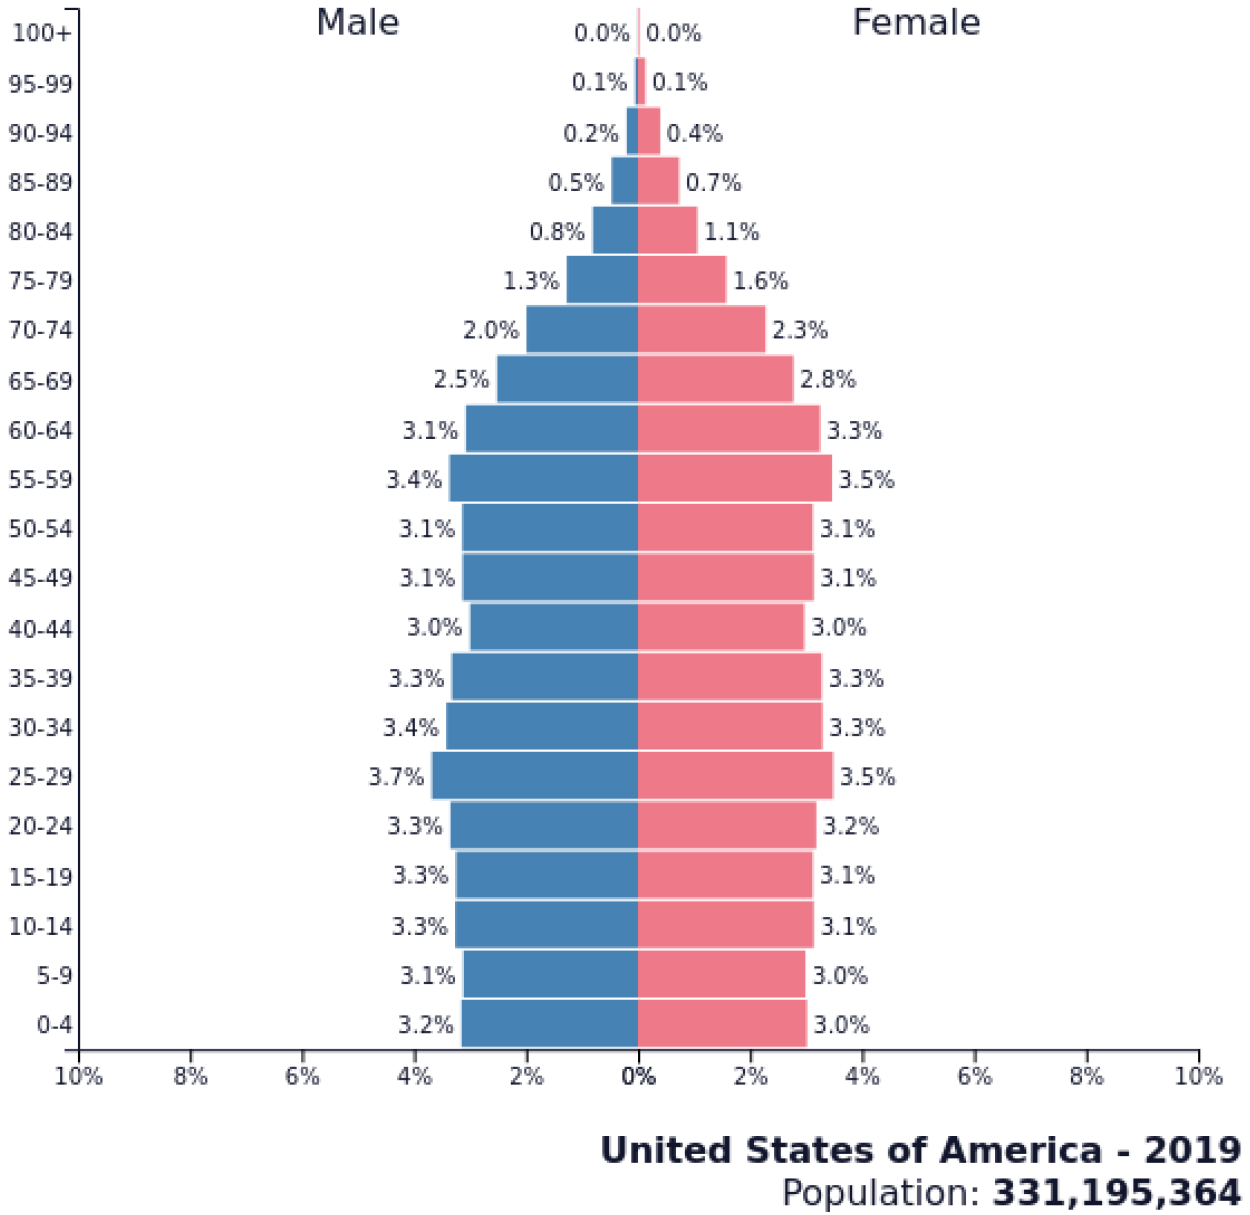
\includegraphics[width=.35\textwidth]{resources/campana-demografica.png}
        \vspace{-0.5cm}
    \end{wrapfigure}
    \textbf{Campana}

    \begin{itemize}
        \item Tasso di fecondità pari a circa 2.1 figli per donna;
        \item Speranza di vita alta, tassi di mortalità relativamente alti a partire dalla terza età;
        \item Popolazione stabile.
    \end{itemize}
    \wrapfill

    %=== URNA ===
    \setlength{\intextsep}{0pt}%
    \begin{wrapfigure}{l}{.35\textwidth}
        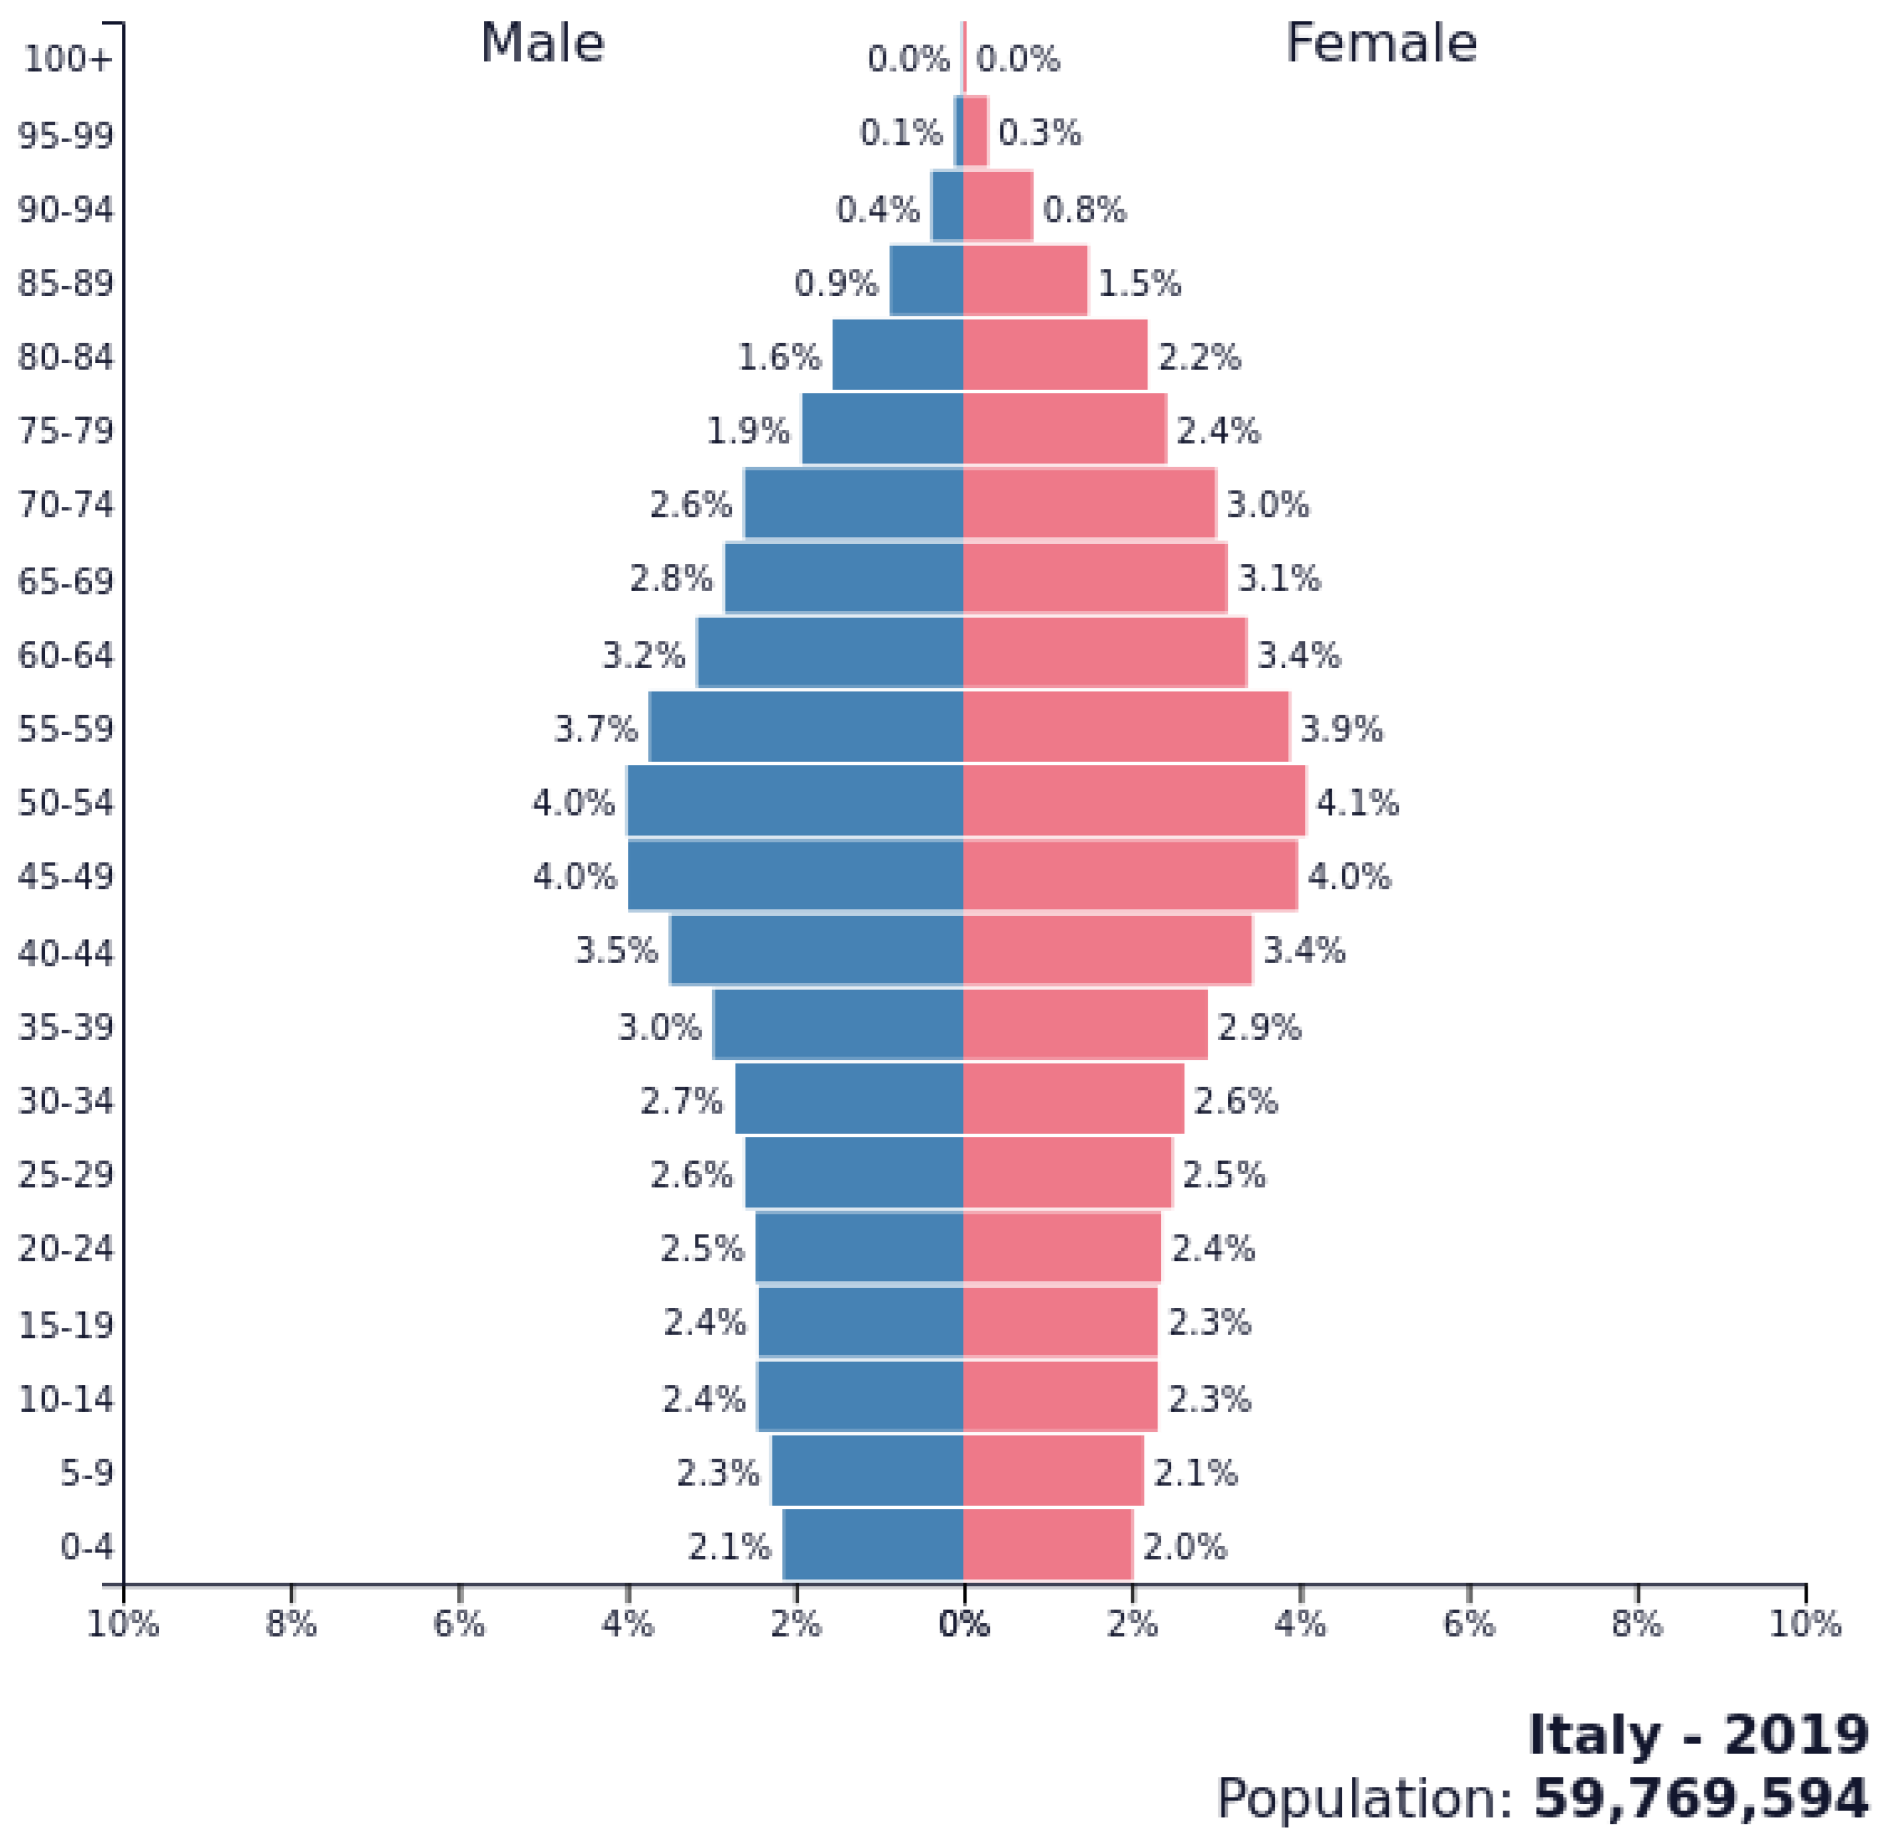
\includegraphics[width=.35\textwidth]{resources/urna-demografica.png}
        \vspace{-0.5cm}
    \end{wrapfigure}
    \textbf{Urna}

    \begin{itemize}
        \item Tasso di fecondità bassi (meno di 2.1 figli per donna);
        \item Alta percentuale di persone anziane, speranza di vita alta, tassi di mortalità alti
            dalla terza età;
        \item Popolazione in diminuzione e in invecchiamento.
    \end{itemize}
    \wrapfill
\end{snippet}

\end{document}